\documentclass[11pt]{article}
\usepackage{xargs}                      % Use more than one optional parameter in a new commands
\usepackage{xcolor}  % Coloured text etc.
\usepackage{pgfgantt}
\usepackage{mathtools}
\usepackage{hyperref}
\usepackage{float}
\usepackage[toc,page]{appendix}
\usepackage[british]{babel}
\usepackage{minted}
\usepackage[bibstyle=numeric, backend=biber, sorting=none]{biblatex}
\addbibresource{../Meine Bibliothek.bib}
%
\usepackage[colorinlistoftodos,prependcaption,textsize=tiny]{todonotes}

\newcommand{\defeq}{\vcentcolon=}
\newcommandx{\unsure}[2][1=]{\todo[linecolor=red,backgroundcolor=red!25,bordercolor=red,#1]{#2}}
\newcommandx{\change}[2][1=]{\todo[linecolor=blue,backgroundcolor=blue!25,bordercolor=blue,#1]{#2}}
\newcommandx{\info}[2][1=]{\todo[linecolor=OliveGreen,backgroundcolor=OliveGreen!25,bordercolor=OliveGreen,#1]{#2}}
\newcommandx{\improvement}[2][1=]{\todo[linecolor=Plum,backgroundcolor=Plum!25,bordercolor=Plum,#1]{#2}}
\newcommand{\code}[1]{\texttt{#1}}
%Gummi|065|=)
\title{\textbf{Exposé Masterarbeit}}
\author{Carsten Csiky}
\date{}
\begin{document}

\maketitle

\section{Abstract}


Software correctness is a central goal for software development.
One way to improve correctness is using strong and descriptive types and verifying them with type systems.
In particular Refinement Types demonstrated, that even with a verification system that is restricted to a decidable logic, intricate properties can be expressed and verified in a lightweight and gradual way.
However existing approaches for adapting Refinement Types from functional to imperative languages proved hard without compromising on at least one of core features of Refinement Types.
% I argue that a base language restricted to unique mutable references will make
This thesis aims to design a Refinement Type system without such compromises by taking advantage of Rust's restriction to unique mutable references. 
I will define a Refinement Type language and typing rules and argue for their soundness. Additionally I will implement a prototype verifier to evaluate the effectiveness of the approach on selected examples.


% \todo{zu konkret: stattdessen vorgehensweise}

\section{Defining the Goal}

The goal of the thesis is to show that Refinement Types can be idiomatically adapted to languages with unique mutable references. It aims to enable gradual adoption of lightweight verification methods in mutable languages.

I aim for automated parsing of refinement types and verification.
In case implementing these translations could not be completed, the use cases will be transformed manually.
In addition, a description of the syntax and semantics of the constructs, that will extend Rust's type system, will be provided as well as justification for their soundness. A feasibility study on minimal examples of representative use cases will show how useful the proposed verification system is. For use cases that could not be covered by the proposed additions, the reason will be investigated.

Specifying or verifying complete Rust modules or the entire Rust language is not the goal of the thesis. In particular \code{unsafe} Rust will not be taken into account in specification nor implementation. Implementing Liquid Type inference in also not a goal of the thesis.


\section{Exposition}

\subsection{Why?}

% With increasing reliance on increasingly complex software, ensuring correctness of programs is a vital concern to software development.
With increasing amount and reliance of software, ensuring the correctness of programs is a vital concern for the future of software development.
Although research in this area has made good progress, most approaches are not accessible enough for general adoption by the developers. Especially in light of a predicted shortage of developers\cite{breaux_2021_2021-1}, it is not sufficient to require developers to undergo year-long training in specialized and complex verification methods to ensure the correctness of their software. It is therefore crucial to integrate with their existing tooling and workflows to ensure the future high quality of software.
One avenue for improving accessability for functional verification is extending the expressiveness of the type system to cover more of the correctness properties.
Using type systems for correctness was traditionally prevalent in purely functional languages where evolving states are often represented by evolving types, offering approachable and gradual adoption of verification methods. Tracing evolving states in the type system would be especially useful for languages with mutability, since substantial parts of the behaviour of the program is expressed as mutation of state. In particular Rust seems like a promising target language, because mutability is already tracked precisely and thus promising functional verification for relatively minimal effort on the programmer's part.

% In systems programming, there has always been an interest in both performance and correctness, as
% these pieces of software are often the foundation of critical infrastructure.

% The classical approaches to ensure correctness include extensive testing, long experience and bmc, because these approaches are approachable to programmers as well as understandable in the programming context (i.e. no separate language)

% Rust -- a relative newcomer to the systems programming field -- has the goal of guaranteeing memory and thread safety at runtime by extending the type system, which works quite well.

% User-defined functional requirements however cannot be checked by Rust's type system and require users to use testing / fuzzing to check for correctness.

% Testing is inadequate in terms of accuracy, while heavy verification systems are inadequate in terms of accessability to developers:
% Both workflow and the specification languages are hard to adapt to existing programming workflows.

% In contrast developers are used to interacting with statically typed languages and their type warnings. It is therefore desirable to embed functional verification systems in type checking phase a compiler.


\subsection{What?}

The thesis will enable automated verification of programs with mutability against refinement type specifications by taking advantage of Rust's strong Ownership Model.

The verification should be sound, decidable and feasible in the identified use cases, which will be tested on minimal -- yet representative -- examples. The examples will include full refinement type annotations, consequently making type inference optional. Listing \ref{lst:pushall} shows how an example program might look like: The \code{ty!} macros specify Refinement Types, which are used in the type checking of the \code{client} function for detect an index out of bounds error.


\begin{listing}
	\inputminted[fontsize=\footnotesize]{rust}{./pushall.rs}
	\caption{Example Use-Case: \code{push\_all} specifies how the \code{Vec} length changes by calling it; as a result \code{client} should not compile.}
	\label{lst:pushall}
\end{listing}

Additionally justification for why the refinement types system is sound will be provided.
The specification will be written in an extension of the Rust type language, inspired by refinement types.


\subsection{How?} \label{ssec:How}

This section starts with outlining the fundamental ideas (denoted "T1" to "T5") the thesis will be based on.

% todo add deliverables
\begin{itemize}
	\item[T1] Identify the relevant concepts (like mutable, immutable and owned types) and their semantics. The deliverable is a set of minimal -- yet representative -- examples, with explanations for why they are representative.
	\item[T2] Devise a Refinement Type system that covers the relevant concepts, in particular mutable but unique references. Refinement types are inherently limited in expressiveness, thusly in cases where use cases cannot be covered, the reason will be explained. The result is a concrete description of the syntax and type judgment semantics.
	\item[T3] Justify why the type system is sound and investigate its limitations. If necessary for the use cases, a definition of suitable axioms for language build-in types will be added. The deliverables is a set of refinement type coercions.
	\item[T4] Develop a prototype for translating refinement type judgments to a verification backend. The deliverable is a parser for Refinement Types and a tool for transformation of to a verification backend or alternatively a description of the process.
	\item[T5] Conduct a feasibility study on different categories of common use cases. The result is a set of proven examples. If some examples could not be proven, the reason will be investigated and explained.
\end{itemize}

Instead of conducting these tasks once for all use cases the set of tasks will be performed incrementally on the identified use cases in order of increasing complexity. These steps are denoted "S1" to "S7". These steps are connected to specific time in Section \ref{sec:schedule}.

\begin{itemize}
	\item[S1] \textbf{Fundamentals}: Cover the mutable, immutable and owned variables, which are specified with (non-abstract) refinement types. In terms of the value-level language, this step will cover assignments, if statements and tuples or product types.
	\item[S2] \textbf{Modular Verification}: Extend the system to cover modular verification. This entails propagating type information between caller and callee. Consequently, the value-level language will be extended with function calls.
	\item[S3] \textbf{Loops}: This step adds loops to the value-level language necessitating the handling of loop invariants (or an  alternative thereof). The invariants will not be automatically inferred.
	\item[S4] \textbf{Predicate Generics}: Improve the expressivity of the type system by adding abstract refinement
	\item[S5] \textbf{ADTs}: This step would consist of extending the type system with sum types and the language with pattern matching, as well as extending the specification with means of expressing restrictions on sum type variants.
	\item[S6] \textbf{Higher-Order Functions}: Extend the system with non-capturing lambdas and their refinement type specification. Completing this step is optional.
	\item[S7] \textbf{Concurrency}: Explore how this approach can be expanded to cover concurrent programs. Starting this step is optional.
\end{itemize}

\section{State of the Art}

There currently does not exist an implementation of refinement types for Rust.

Relevant papers originate from two lines of work. Firstly additions to refinement types for mutability, asynchronous execution etc. and secondly other verification frameworks for Rust.

For example, Lanzinger \cite{lanzinger_property_2021} successfully adapted refinement types to Java, which allows the user to check, that property types described by java annotations hold true throughout the program. At this point in time, specification and verification is limited to immutable (\code{final}) data.

Kloos et al. \cite{kloos_asynchronous_2015} extended refinement types to mutable and asynchronous programs. The paper explores how changes to possibly aliased memory cells can be tracked throughout a OCaml program. For that purpose the types are extended by a set of requirements on memory objects, which track distinctness and refined types of these memory cells. In contrast to OCaml, Rust already guarantees that mutable memory is not aliased and in particular \textit{all mutable memory locations must be accessible by a variable name in the current context}, which offers substantial advantages in terms of simplicity to specification and verification of Rust programs.

In terms of alternative verification approaches, Prusti\cite{astrauskas_leveraging_2019} is notable, because of their work on formalizing the full Rust semantics, including \code{unsafe}. Prusti is a heavy-weight functional verification framework for Rust; based on separation logic.

Alternative verification approaches also exists: For example RustHorn\cite{matsushita_rusthorn_2020} employs constrained horn clauses based verification to Rust. Particularity relevant for this thesis is the novel formalization for mutable references used in the paper. The authors stipulate that mutable references should be specified by a pre- and post-state from before a reference is borrowed to after it is returned.

\section{Schedule} \label{sec:schedule}

This sections describes the relation of the steps from Section \ref{ssec:How} to their timeslot and the dependencies between them in form of a gantt diagram. There are one milestones, namely completion of the critical stages, which is denoted \textit{Feature Complete}.


\begin{ganttchart}[
	time slot format=isodate,
	x unit=0.04cm,
	today = 2022-03-10,
	link bulge=2.5,
	]{2022-03-10}{2022-09-15}
\gantttitlecalendar{year, month=shortname} \\

\ganttbar[name=S1]{S1 Fundamentals}{2022-03-10}{2022-03-24} \\

\ganttbar[name=S2]{S2 Modular}{2022-03-30}{2022-04-14} \\

\ganttbar[name=S3]{S3 Loops}{2022-04-08}{2022-05-08} \\
\ganttlink[link mid=0.1]{S1}{S3}



\ganttbar[name=S4]{S4 Predicate Generics}{2022-05-08}{2022-05-30}\\
\ganttlink[link mid=0.2]{S2}{S4}


\ganttbar[name=S5]{S5 ADTs}{2022-05-30}{2022-06-18}  \\
\ganttlink[link mid=0.01]{S1}{S5}

\ganttlinkedmilestone[name=fc]{Feature Complete}{2022-06-18} \\
\ganttlink[]{S4}{fc}


\ganttbar[name=S6]{S6 Higher-Order}{2022-06-28}{2022-07-25} \\
\ganttlink[link mid=0.25]{S4}{S6}



\ganttbar[name=S7]{S7 Concurrency}{2022-07-25}{2022-08-10} \\
\ganttlink[link mid=0.5]{S6}{S7}


\ganttbar[name=raw_version]{Draft Version}{2022-06-10}{2022-08-15} \\
	\ganttlinkedbar[name=corrections]{Revisions}{2022-08-15}{2022-09-06} \\
		\ganttlinkedbar{Buffer}{2022-09-06}{2022-09-15} \\

\end{ganttchart}

\newpage
\begin{appendices}

\section{Use Case Analysis}

To gain some understanding of how relevant mutability is in Rust, all published Rust crates (Rusts version packages) published on crates.io with at least 10 versions were analysed\footnote{The limit of 10 versions is used to eliminate inactive and placeholder packages}. The analysis uses the syntactical structure to infer mutability information about the following various AST items:
\begin{itemize}
	\item Local Variable Definitions. These can be tracked with high confidence
	\item Parameters, which are considered immutable if they are passed as immutable references or owned.
	\item Function Definitions, which are considered immutable, iff all parameters considered immutable.
	\item Arguments. Hard to track
	\item Function Calls, which are considered immutable, iff all arguments are considered immutable.
\end{itemize}
A total of around 52 million items were found in 228263 files in a combined code-base size of over 64 million lines of Rust code (without comments and white space lines)\footnote{Calculated with \texttt{cloc}}

% from cloc
% ----------------------------------------------------------------------------------------
% Language                              files          blank        comment           code
% ----------------------------------------------------------------------------------------
% Rust                                 228263        5664979       10317162       64193670
% C                                     32945        1539542        1979846       13468919
% C++                                   18084        1263696        1093652        7956897
% JSON                                  15838           1897              0        6424252
% C/C++ Header                          31619        1152322        2015896        6284146
% XML                                    5142          25277          25773        4807556
% Assembly                               4146         534785         582345        2631991


Figure~\ref{fig:mutabillity_by_category} shows the ratio of mutable to immutable items. Note that about 30\% of local variables are defined mutable while just 10\% to 20\% of parameters are mutable and less than 10\% of functions have mutable parameters at all.

\begin{figure}[H]
	\centering
	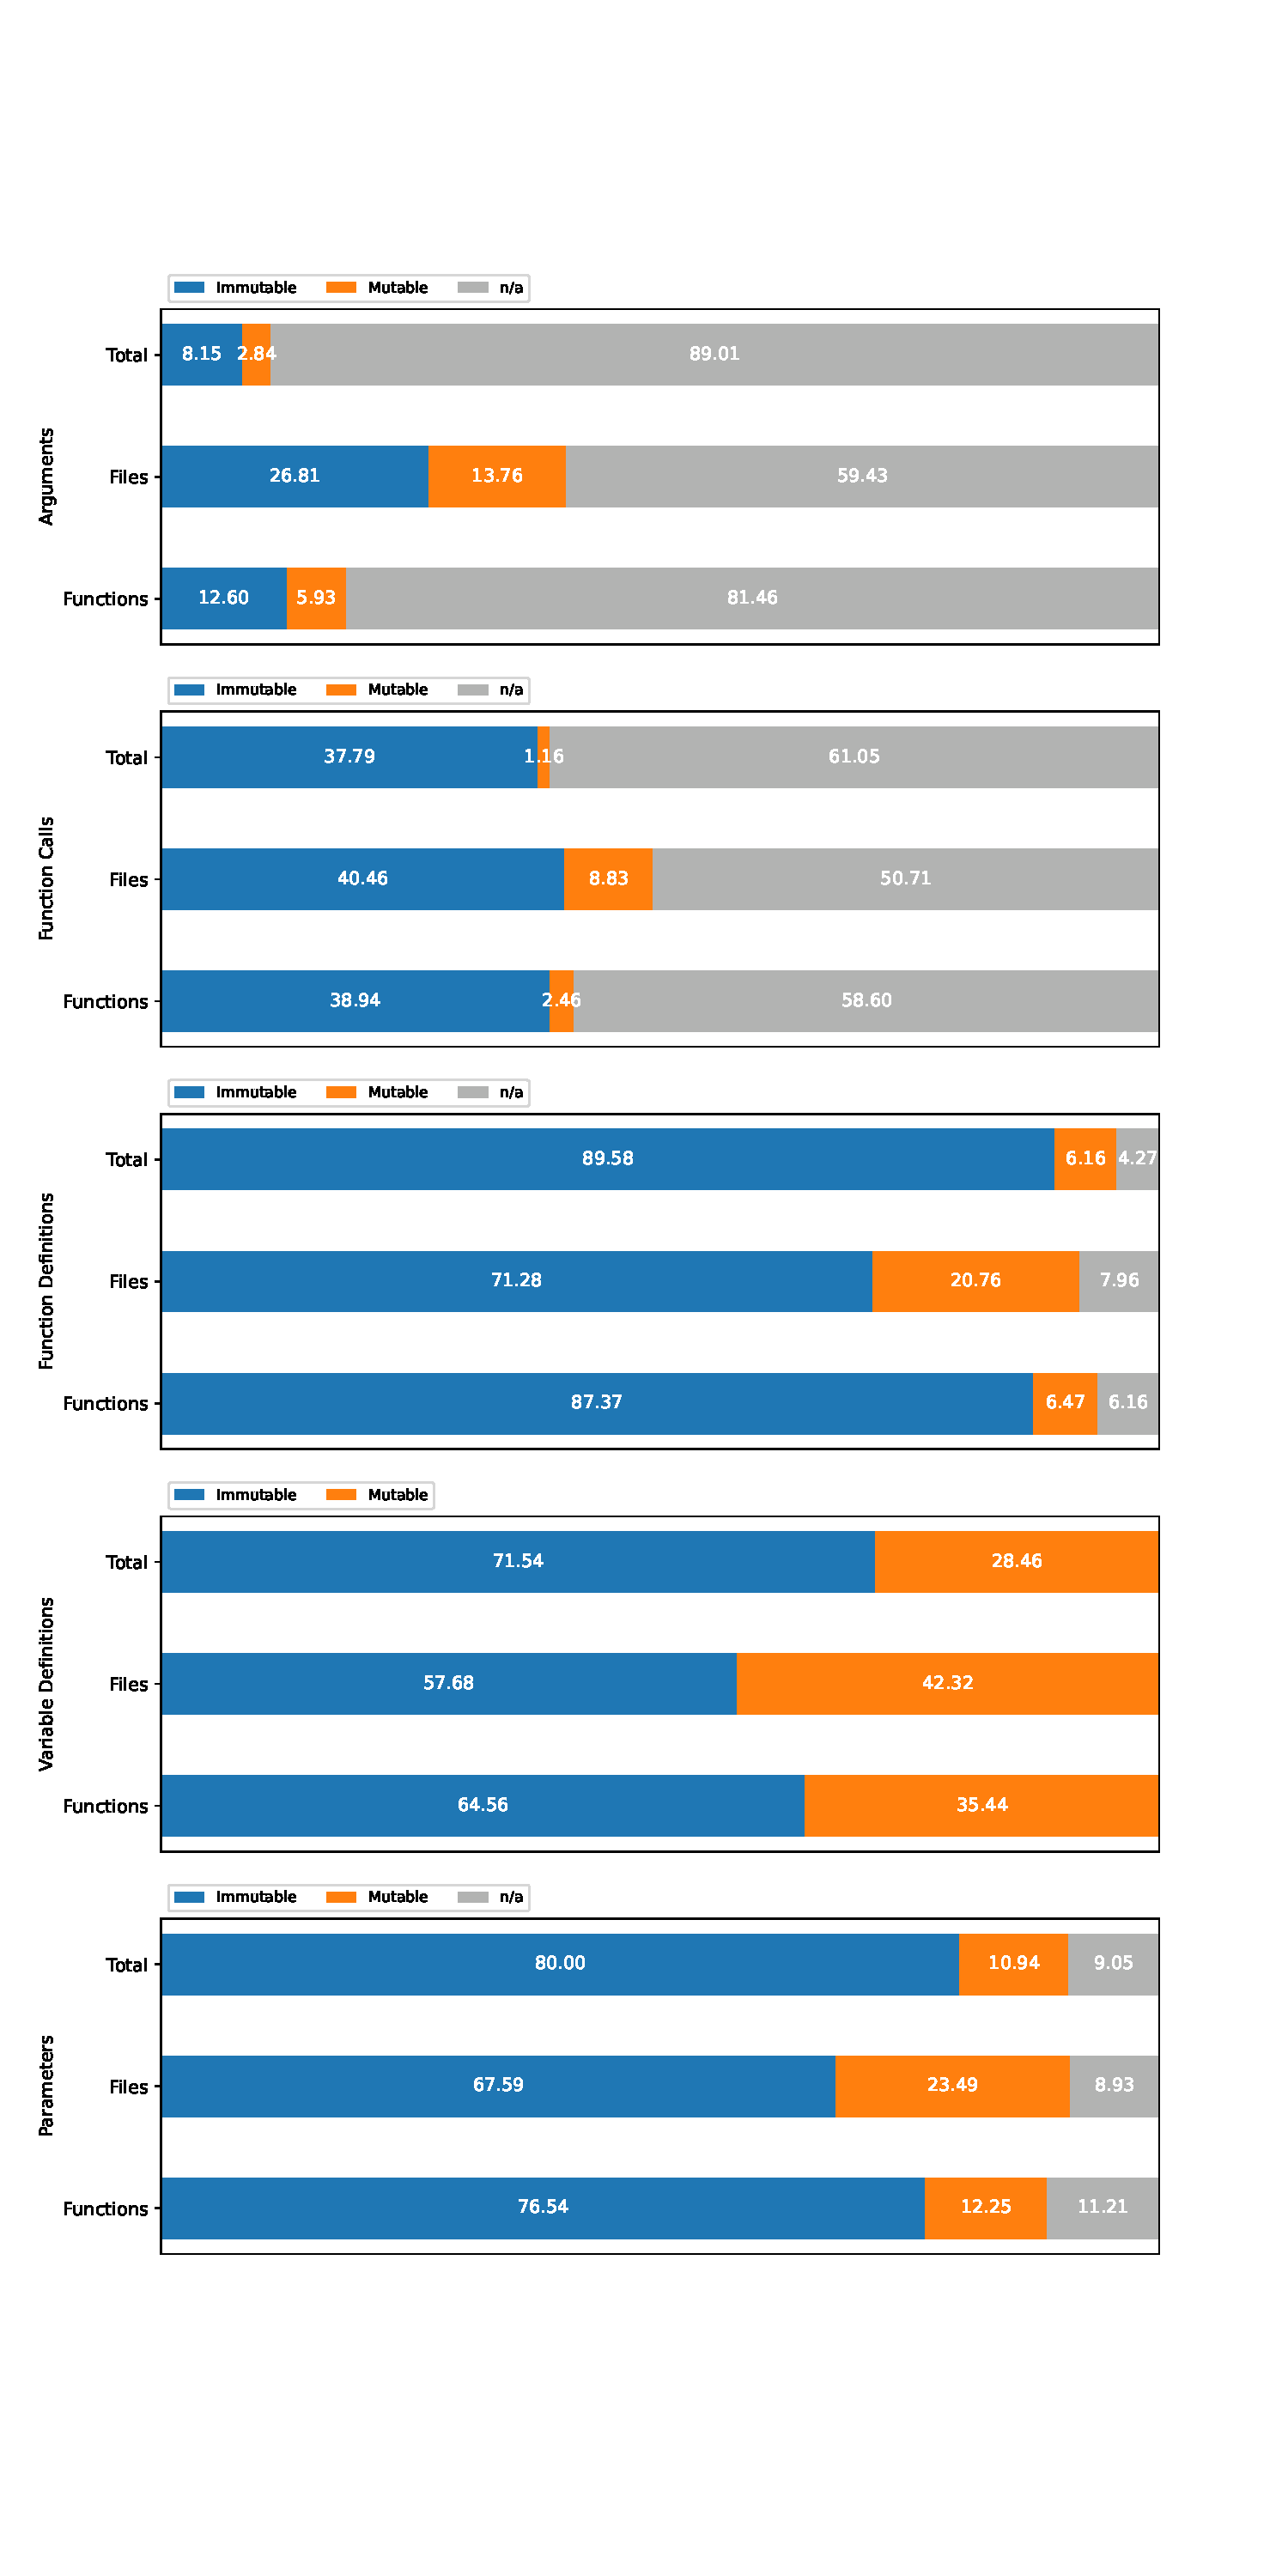
\includegraphics[width=0.9\linewidth, clip, trim={0.5cm 6cm 0.5cm 6cm}]{../mutability_by_category.pdf}
	\caption{Ratio of Immutable to Mutable Versions of Different AST Items. Items are Counted by Unique Occurrences}
	\label{fig:mutabillity_by_category}
\end{figure}


\end{appendices}


\printbibliography

\end{document}
